\documentclass[11pt]{article}
% Build: cd paper && latexmk -pdf main.tex   (tables/numbers: python3 paper/tables.py; figures: python3 scoring/figures.py)
\usepackage[a4paper,margin=2.5cm]{geometry}
\usepackage[utf8]{inputenc}
\usepackage[T1]{fontenc}
\usepackage{lmodern}
\usepackage{amsmath}
\usepackage{booktabs}
\usepackage{graphicx}
\usepackage{xcolor}
\usepackage{lineno}
\sloppy
\usepackage[numbers,sort&compress]{natbib}
\usepackage{url}
\usepackage[hidelinks]{hyperref}
\urlstyle{same}
\usepackage{setspace}
\onehalfspacing
\linenumbers

% generated by paper/tables.py - do not edit
\newcommand{\numToneAzeroN}{10}
\newcommand{\numToneAzeroAcc}{93.21}
\newcommand{\numToneAzeroAccSD}{1.13}
\newcommand{\numToneAzeroCost}{0.38}
\newcommand{\numToneAzeroWall}{3.1}
\newcommand{\numToneAzeroDistinct}{7}
\newcommand{\numToneAzeroDistinctFiles}{10}
\newcommand{\numToneAzeroUnscorable}{0}
\newcommand{\numToneAzeroAccPostHoc}{93.21}
\newcommand{\numToneAoneN}{10}
\newcommand{\numToneAoneAcc}{78.58}
\newcommand{\numToneAoneAccSD}{41.41}
\newcommand{\numToneAoneCost}{0.73}
\newcommand{\numToneAoneWall}{5.2}
\newcommand{\numToneAoneDistinct}{6}
\newcommand{\numToneAoneDistinctFiles}{10}
\newcommand{\numToneAoneUnscorable}{2}
\newcommand{\numToneAoneAccPostHoc}{98.22}
\newcommand{\numToneAonePmxRuns}{0}
\newcommand{\numToneAonePmxKnown}{10}
\newcommand{\numToneAonePmxHttpRuns}{0}
\newcommand{\numToneAtwoN}{10}
\newcommand{\numToneAtwoAcc}{98.65}
\newcommand{\numToneAtwoAccSD}{0.06}
\newcommand{\numToneAtwoCost}{0.50}
\newcommand{\numToneAtwoWall}{3.8}
\newcommand{\numToneAtwoDistinct}{9}
\newcommand{\numToneAtwoDistinctFiles}{10}
\newcommand{\numToneAtwoUnscorable}{0}
\newcommand{\numToneAtwoAccPostHoc}{98.65}
\newcommand{\numToneAthreeN}{10}
\newcommand{\numToneAthreeAcc}{98.64}
\newcommand{\numToneAthreeAccSD}{0.00}
\newcommand{\numToneAthreeCost}{0.20}
\newcommand{\numToneAthreeWall}{1.2}
\newcommand{\numToneAthreeDistinct}{1}
\newcommand{\numToneAthreeDistinctFiles}{5}
\newcommand{\numToneAthreeUnscorable}{0}
\newcommand{\numToneAthreeAccPostHoc}{98.64}
\newcommand{\numToneAfourN}{10}
\newcommand{\numToneAfourAcc}{98.64}
\newcommand{\numToneAfourAccSD}{0.00}
\newcommand{\numToneAfourCost}{0.09}
\newcommand{\numToneAfourWall}{1.1}
\newcommand{\numToneAfourDistinct}{1}
\newcommand{\numToneAfourDistinctFiles}{4}
\newcommand{\numToneAfourUnscorable}{0}
\newcommand{\numToneAfourAccPostHoc}{98.64}
\newcommand{\numToneAtwoVsAoneDiff}{+20.08}
\newcommand{\numToneAtwoVsAoneCI}{+0.40 to +49.52}
\newcommand{\numToneAthreeVsAoneDiff}{+20.06}
\newcommand{\numToneAthreeVsAoneCI}{+0.38 to +49.52}
\newcommand{\numToneAthreeVsAtwoDiff}{$-$0.01}
\newcommand{\numToneAthreeVsAtwoCI}{$-$0.05 to +0.02}
\newcommand{\numToneAfourVsAthreeDiff}{+0.00}
\newcommand{\numToneAfourVsAthreeCI}{+0.00 to +0.00}
\newcommand{\numToneAzeroVsAthreeDiff}{$-$5.43}
\newcommand{\numToneAzeroVsAthreeCI}{$-$6.02 to $-$4.73}
\newcommand{\numTtwoAzeroN}{10}
\newcommand{\numTtwoAzeroAcc}{--}
\newcommand{\numTtwoAzeroAccSD}{--}
\newcommand{\numTtwoAzeroCost}{0.23}
\newcommand{\numTtwoAzeroWall}{3.3}
\newcommand{\numTtwoAzeroDistinctFiles}{10}
\newcommand{\numTtwoAoneN}{2}
\newcommand{\numTtwoAoneAcc}{--}
\newcommand{\numTtwoAoneAccSD}{--}
\newcommand{\numTtwoAoneCost}{0.65}
\newcommand{\numTtwoAoneWall}{3.0}
\newcommand{\numTtwoAoneDistinctFiles}{2}
\newcommand{\numTtwoAonePmxRuns}{2}
\newcommand{\numTtwoAonePmxKnown}{2}
\newcommand{\numTtwoAonePmxHttpRuns}{0}
\newcommand{\numTthreeaAzeroN}{5}
\newcommand{\numTthreeaAzeroAcc}{92.93}
\newcommand{\numTthreeaAzeroAccSD}{1.60}
\newcommand{\numTthreeaAzeroCost}{0.58}
\newcommand{\numTthreeaAzeroWall}{4.1}
\newcommand{\numTthreeaAzeroDistinct}{4}
\newcommand{\numTthreeaAzeroDistinctFiles}{5}
\newcommand{\numTthreebAzeroN}{3}
\newcommand{\numTthreebAzeroAcc}{95.76}
\newcommand{\numTthreebAzeroAccSD}{0.00}
\newcommand{\numTthreebAzeroCost}{0.53}
\newcommand{\numTthreebAzeroWall}{3.7}
\newcommand{\numTthreebAzeroDistinct}{3}
\newcommand{\numTthreebAzeroDistinctFiles}{3}
\newcommand{\numTthreecAzeroN}{5}
\newcommand{\numTthreecAzeroAcc}{93.63}
\newcommand{\numTthreecAzeroAccSD}{2.64}
\newcommand{\numTthreecAzeroCost}{0.63}
\newcommand{\numTthreecAzeroWall}{3.9}
\newcommand{\numTthreecAzeroDistinct}{3}
\newcommand{\numTthreecAzeroDistinctFiles}{5}
\newcommand{\numTthreedAzeroN}{5}
\newcommand{\numTthreedAzeroAcc}{100.00}
\newcommand{\numTthreedAzeroAccSD}{0.00}
\newcommand{\numTthreedAzeroCost}{0.12}
\newcommand{\numTthreedAzeroWall}{0.9}
\newcommand{\numTthreedAzeroDistinctFiles}{5}
\newcommand{\numTthreedAoneN}{5}
\newcommand{\numTthreedAoneAcc}{93.33}
\newcommand{\numTthreedAoneAccSD}{14.91}
\newcommand{\numTthreedAoneCost}{0.18}
\newcommand{\numTthreedAoneWall}{1.0}
\newcommand{\numTthreedAoneDistinctFiles}{5}
\newcommand{\numTthreedAonePmxRuns}{0}
\newcommand{\numTthreedAonePmxKnown}{5}
\newcommand{\numTthreedAonePmxHttpRuns}{0}
\newcommand{\numTthreeeAzeroN}{5}
\newcommand{\numTthreeeAzeroAcc}{93.21}
\newcommand{\numTthreeeAzeroAccSD}{1.05}
\newcommand{\numTthreeeAzeroCost}{0.56}
\newcommand{\numTthreeeAzeroWall}{3.8}
\newcommand{\numTthreeeAzeroDistinct}{4}
\newcommand{\numTthreeeAzeroDistinctFiles}{5}
\newcommand{\numToneAtwoVsAonePostHocDiff}{+0.43}
\newcommand{\numToneAtwoVsAonePostHocCI}{+0.35 to +0.52}
\newcommand{\numToneAthreeVsAonePostHocDiff}{+0.42}
\newcommand{\numToneAthreeVsAonePostHocCI}{+0.35 to +0.51}
\newcommand{\numToneAoneAccIsolated}{70.17}
\newcommand{\numToneAoneNIsolated}{7}
\newcommand{\numToneAoneAccUser}{98.18}
\newcommand{\numToneAoneNUser}{3}
\newcommand{\numToneAtwoVsAoneIsolatedDiff}{+28.48}
\newcommand{\numToneAtwoVsAoneIsolatedCI}{+0.38 to +56.61}
\newcommand{\numToneAthreeVsAoneIsolatedDiff}{+28.47}
\newcommand{\numToneAthreeVsAoneIsolatedCI}{+0.38 to +56.58}
\newcommand{\numToneAtwoVsAoneUserDiff}{+0.47}
\newcommand{\numToneAtwoVsAoneUserCI}{+0.34 to +0.67}
\newcommand{\numToneAthreeVsAoneUserDiff}{+0.46}
\newcommand{\numToneAthreeVsAoneUserCI}{+0.35 to +0.67}


\title{Do agentic pharmacometrics tools need server infrastructure?\\
\large A controlled benchmark of an MCP platform versus Agent Skills for noncompartmental analysis and PK workflows}
\author{Dhruvik Pandya\\[4pt]
\small Department of Pharmacology, All India Institute of Medical Sciences (AIIMS), Jodhpur, India\\
\small Corresponding author: Dhruvik Pandya, \href{mailto:pandyadhruvik18@gmail.com}{pandyadhruvik18@gmail.com}}
\date{}

\begin{document}
\maketitle

\begin{abstract}
\noindent\textbf{Background.} PMxAgent makes LLM-agent pharmacokinetic analyses reproducible with a server stack
(Docker, an R Plumber API and a Model Context Protocol (MCP) server) that exposes validated R functions as tools. Which
part of that design gives its accuracy and reproducibility has not been tested.

\noindent\textbf{Methods.} We re-ran PMxAgent's noncompartmental analysis (NCA) benchmark (182 drugs, 1,820 subjects,
PKanalix reference) in one client (Claude Code) and one model, varying only what the agent was given: nothing (A0); PMxAgent 1.0.0 over MCP (A1); Agent Skills with NCA instructions only (A2); the same
Skills plus a bundled, tested PKNCA script (A3); A3 on a smaller model (A4); and, post hoc, A1 plus PMxAgent's
instruction file (A1b). We also ran PMxAgent's simulation case study (T2) and five stress tasks (T3).

\noindent\textbf{Results.} Overall accuracy was \numToneAzeroAcc\% for A0, \numToneAoneAcc\% for A1,
\numToneAtwoAcc\% for A2 and \numToneAthreeAcc\% for A3 and A4. The A1 agent called a PMxAgent tool in
\numToneAonePmxRuns\ of \numToneAonePmxKnown\ runs, and \numToneAoneUnscorable\ of its runs named the drug but not the
subject and scored 0. A2$-$A1 was \numToneAtwoVsAoneDiff\ percentage points (95\% CI \numToneAtwoVsAoneCI), and
\numToneAtwoVsAonePostHocDiff\ (\numToneAtwoVsAonePostHocCI) without those runs (post hoc). A1b scored
\numToneAonebAcc\%. Only the arms that executed a fixed script gave identical parameter values in every run, at
\$\numToneAthreeCost\ (A3) and \$\numToneAfourCost\ (A4) per run against \$\numToneAoneCost\ for A1. On four NCA stress
tasks A3 gave one set of values per task and was equivalent to or more accurate than A1; the smaller model matched it
on two. Over the five NCA tasks the A1 agent called a PMxAgent tool in \numNcaAonePmxRuns\ of \numNcaAonePmxKnown\ runs.
In T2, A3 runs that used the packaged parameter set and script gave an identical EC$_{50}$; A1 runs with the same
parameters and seed did not.

\noindent\textbf{Conclusions.} On PMxAgent's NCA benchmark and four harder NCA inputs, accuracy came from domain
instructions and identical parameter values from a fixed script with the larger model; neither required the server stack. In simulation,
fixed code gave identical values only when the steps around it were fixed too. Offered PMxAgent's tools alone, the agent
rarely used them for NCA, so PMxAgent's own reproducibility was not tested. MCP remains useful for client-agnostic,
validated, multi-user deployment.
\end{abstract}

\noindent\textbf{Keywords:} pharmacometrics; noncompartmental analysis; large language models; AI agents;
Model Context Protocol; Agent Skills; reproducibility

% ---------------------------------------------------------------------------------------------------------------
\section{Introduction}
LLMs are being tried across the pharmacometrics workflow: writing NONMEM code
\cite{shin2024nonmem,zheng2025nonmemcoding}, reading model output \cite{cha2025nonmemoutput}, building QSP models
\cite{saini2025qspcopilot} and running pharmacokinetic calculations \cite{shin2023chatgptpk}; see
\cite{tosca2025vision} for a review. A recurring finding is that the output, from numerical results to generated code, differs
between repeats of the same prompt \cite{shin2023chatgptpk,shin2024nonmem}.

PMxAgent \cite{bloomingdale2026pmxagent} answers this by moving the calculations into fixed, validated R functions
(PKNCA \cite{pknca}, mrgsolve \cite{mrgsolve} and others) served by an R Plumber API inside Docker, and exposing them to
the agent as tools through a Model Context Protocol (MCP) server \cite{mcp} generated from the API's OpenAPI
description. On a benchmark of 182 drugs and 1,820 simulated subjects, PMxAgent matched PKanalix \cite{pkanalix} for
98.3\% of subject-parameters and gave identical results across runs, whereas general-purpose agents that wrote new
code each time scored 91.6--98.2\% and varied between runs \cite{bloomingdale2026pmxagent}.

That comparison changes several things at once: the agent client, the model, whether domain rules were given, and
whether calculations ran in fixed code. It cannot say which of these produced the gain. A lighter design can supply the
last two without the others. Agent Skills \cite{agentskills} are folders of instructions and scripts that an agent
loads when a task needs them; they need no server, container or network service, and they are a packaged form of the
``context engineering'' recently described for pharmacometric tasks \cite{pritchardbell2026context}. If accuracy comes
from the NCA rules and reproducibility from running a fixed script, Skills should match an MCP platform with far less
infrastructure.

We asked which of three ingredients (domain instructions, a fixed script or a server stack) produces PMxAgent's accuracy
and run-to-run identity. We held the client, the model and the prompt fixed, varied only what the agent was given
(Figure~\ref{fig:arch}), and ran PMxAgent's own NCA benchmark, its simulation case study and five harder tasks.

% ---------------------------------------------------------------------------------------------------------------
\section{Methods}
\subsection{Benchmark and scoring}
Task~1 (T1) is the NCA benchmark from the PMxAgent supporting information \cite{bloomingdale2026pmxagent}: 182 drugs,
1,820 simulated single-dose subjects (IV bolus or extravascular), with PKanalix 2024R1 results as the reference. The
prompt was used verbatim. A fixed suffix, identical in all arms, told the agent to work autonomously, read inputs from
\texttt{inputs/} and write outputs to \texttt{output/}; A1 also received the path under which its tools see the files.

We re-implemented the paper's metric \cite{bloomingdale2026pmxagent}: a subject-parameter is correct if it is within
1\% of PKanalix. $C_\mathrm{max}$, $t_\mathrm{max}$ and AUC$_\mathrm{last}$ are scored for all subjects; the
$\lambda_z$-dependent parameters (AUC$_{\infty,\mathrm{obs}}$, $t_{1/2}$, CL or CL/F, $V_z$ or $V_z$/F) only for
subjects whose PKanalix adjusted $R^2$ is at least 0.80. Overall accuracy is the mean of the seven parameter
accuracies; missing values count as incorrect. Before any run, our scorer reproduced the overall accuracies of the
paper's five published result files exactly (maximum absolute difference 0.00 percentage points). It picks the output
file by coverage of the reference subjects and parameters, never by accuracy, and maps parameter-name spellings
without changing values. A completed run whose results could not
be matched to any reference subject (for example, rows identified by drug only) scored 0, as pre-specified. For A1 we
counted, from each transcript, the agent's calls to PMxAgent tools.

\subsection{Arms}
All arms used Claude Code \cite{claudecode} in headless mode, with one pinned version per task (2.1.283 for T1,
2.1.310 for T2 and T3). A0--A3 used \texttt{claude-sonnet-4-6}, the model behind PMxAgent's published results; A4 used
\texttt{claude-haiku-4-5-20251001}.
\begin{description}
\item[A0] No Skills, no MCP server: the agent writes its own code.
\item[A1] PMxAgent 1.0.0 MCP server (Docker images pinned by digest), as published.
\item[A1b] Secondary arm, T1 only, post hoc: A1 plus the \texttt{CLAUDE.md} instruction file shipped with PMxAgent
1.0.0 (pinned by SHA-256), which Claude Code loads at session start when run in PMxAgent's repository, as its
documentation advises; the prompt was unchanged. The file describes the NCA tool's multi-drug and mixed-route input,
which the tool's API description omits. PMxAgent's authors wrote it for this benchmark's workflow; it contains no
reference values.
\item[A2] Agent Skills, knowledge only: the \texttt{SKILL.md} method instructions (AUC rule, $\lambda_z$ selection,
derived parameters, route and BLQ handling, units, output checks), with all script sections removed.
\item[A3] The same Skills plus a bundled R script (\texttt{run\_nca.R}, PKNCA 0.12.1) that the instructions tell the agent to
call instead of writing NCA code.
\item[A4] A3 with the smaller model.
\end{description}

\begin{figure}[t]
\centering
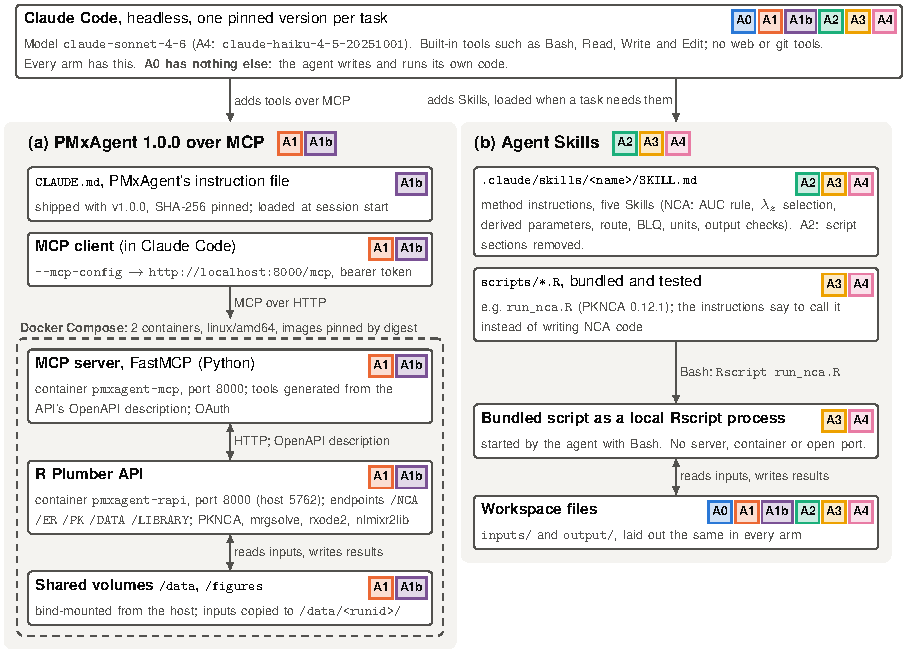
\includegraphics[width=\linewidth]{figures/fig_arch.pdf}
\caption{What each arm gives the agent. Every arm runs Claude Code with its built-in tools; A0 has nothing else, so
the agent writes and runs its own code. (a) A1 adds the tools of PMxAgent 1.0.0 over MCP, served by two Docker
containers; A1b also loads PMxAgent's \texttt{CLAUDE.md}. (b) A2 adds the Skills' instructions only; A3 and A4 add the
bundled scripts, which the agent runs as a local R process. Labelled boxes mark the arms that have each component
(colours as in Figures~\ref{fig:params} and~\ref{fig:cost}). PMxAgent's components are named from its paper
\cite{bloomingdale2026pmxagent} and its Docker and README files.}
\label{fig:arch}
\end{figure}

We wrote five Skills (NCA, PK simulation, data standardisation, exposure--response, model library) from package
documentation and general NCA conventions, without reading PMxAgent's endpoint code. They were tested with
\texttt{testthat} against analytical solutions only and frozen by SHA-256 hash before any benchmark run. The NCA
script was run once on the T1 input to confirm that it completed; its output was not compared with PKanalix before the
freeze. The runner refused to start A2--A4 if any hash differed.

A script counted each stack's infrastructure from its repository (PMxAgent at tag \texttt{v1.0.0}; the frozen
Skills): containers, host ports, services that must run before the agent starts, setup steps (for PMxAgent, those in
its README), and non-blank, non-comment lines by role, excluding documentation and licence files.

\subsection{Run protocol and isolation}
Each run was a new \texttt{claude -p} process in a new git worktree that contained only the task inputs and, for
A2--A4, that arm's Skills, outside the project repository, so no reference data were reachable. User-level settings,
plugins, hooks and automatic memory were disabled, MCP servers were restricted to the arm's configuration, git and web
tools were disallowed, and finished runs were moved to a non-listable archive. An audit of every tool call in all
transcripts found no access to another run's files. One known leak, the user-global
instruction file (general tool-usage rules, no pharmacometric content), was loaded in every T1 run except A1 runs 4--10
and all A1b runs, which ran with no user instructions.

The planned number of runs was 10 per arm for T1 and T2 and 5 per arm for T3. A1 first had 3 T1 runs, because of cost
and time, and was later topped up to 10 under the stricter isolation; A1 is therefore also reported per isolation
regime, as pre-specified before the top-up. Runs stopped by the subscription's usage limit (HTTP 429) or by an
infrastructure failure (an API or authentication error, or no work done) were repeated; a run in which the agent worked
and then crashed or timed out was scored on what it left. Every counted run was scored, whatever its result. Cost is
Claude Code's list-price estimate from token counts.

T2 and T3 runs loaded no user instructions and were made with at most two sessions at a time, spread over two
subscription accounts. PMxAgent's tools write to shared folders, so A1 runs of T2 and T3 made before those folders
were emptied between runs could see earlier runs' files; all were excluded and repeated, a decision made from when the
runs were made, before any of their results was looked at.

\subsection{Further tasks}
Task~2 (T2) is the case study from the PMxAgent paper \cite{bloomingdale2026pmxagent}, with its prompt used verbatim:
simulate 60 subjects in three IV dose groups (10, 30 and 100~mg) with a two-compartment model and 30\% between-subject
variability, run NCA on the simulated profiles, and fit a binary exposure--response model with response rates of 0.1,
0.5 and 0.9. The prompt gives no parameter values or units, so each run chose its own; an added sentence asked for a
\texttt{results.json} with group summaries, EC$_{50}$, seed, number of sampling times and typical parameters. With no
reference answer, T2 was reported descriptively, as pre-specified: completion (a \texttt{results.json} with all three
dose groups); internal consistency, the percentage of reported group means (AUC$_\mathrm{last}$, $C_\mathrm{max}$)
within 1\% of the means recomputed from the run's own simulated data (AUC$_\mathrm{last}$ by the linear-up/log-down
rule); and the spread of EC$_{50}$ across runs. Because the prompt names no AUC rule, consistency under either rule was
added before any T2 run was scored, as a sensitivity analysis.

Runs named their files and columns freely, so the T2 scorer finds the simulated data by column-name patterns. A hand
check on \numTtwoParserN\ runs chosen by a fixed rule (the first two valid runs of each arm, and every run the scorer
at first could not read) found one naming gap, the CDISC subject column \texttt{SUBJID}; fixing it changed no value
already computed and let the scorer read \numTtwoParserFixed\ more runs. The scorer then agreed with the hand check in
\numTtwoParserAgree\ of \numTtwoParserN\ runs.

Task~3 (T3) has five variants. Four are built from the T1 benchmark and scored with the T1 metric: T3a, 30 drugs (300
subjects) as an Excel workbook with one sheet per drug, patients in rows, ``$<$LLOQ'' entries and blank cells; T3b, 65
drugs (650 subjects) with below-quantification records and a stated rule (zero before $t_\mathrm{max}$, missing
after), which before any run we confirmed reproduces the PKanalix AUC$_\mathrm{last}$ for all 220 subjects it affects;
T3c, 30 drugs (300 subjects) with concentrations in four units; and T3e, the full benchmark repeated five times (9,100
subjects). Unlike the T1 prompt, these prompts state how each subject must be identified. The fifth, T3d, asks for a
simulation of 20 subjects with a one-compartment oral model (parameters given) and the typical-subject
$C_\mathrm{max}$, $t_\mathrm{max}$ and AUC$_{0-\infty}$, scored as the percentage of these within 1\% of the
analytical solution. PMxAgent's simulation tool covers IV administration only, so T3d lies outside A1's tool set.

\subsection{Statistics}
For each pre-specified pair of arms (A2$-$A1, A3$-$A1, A3$-$A2, A4$-$A3, A0$-$A3) we report the difference in mean
overall accuracy with a 95\% percentile bootstrap CI (10,000 resamples of runs within each arm) and an exact two-sided
permutation $p$-value; arms were equivalent only if the whole CI lay within $\pm$1.0 percentage point. For T2 and T3 the
analysis was fixed in the repository before any of their runs (commit \texttt{08ea7b3}); the comparisons apply to each
NCA stress task and are exploratory for T3d. Reproducibility is the SD of overall accuracy and the number of distinct
sets of parameter values (scored table, six significant digits). The terminal-point match is the percentage of subjects
scored for $\lambda_z$-dependent parameters whose terminal phase used as many points as PKanalix's, pooled over runs
that reported the number of points (a missing count counts as not matching).

Several choices followed some results and are labelled where reported. The T1 comparisons were specified after the
T1 runs. After the T1 scores were seen we added the comparisons without the runs whose results could not be matched to
subjects, and made explicit that each of such a run's seven parameters also scores 0 (no overall score changes). A1b
and its comparisons (A1b$-$A1, A2$-$A1b, A3$-$A1b, A4$-$A1b) were specified before any A1b run but after the A0--A4 T1
results were known; A1b is reported alongside A1, never instead of it. The split of $\lambda_z$-dependent errors by
terminal-point match is descriptive and was decided after all results were seen. For T2, the \texttt{SUBJID} fix
followed the first T2 results, and the EC$_{50}$ spread measure (the number of distinct values and the largest group of
identical values) was chosen after the data were seen, as were the unit conversion (to h$\cdot\mu$g/mL) and 1\% rule
for the planned descriptive comparison with PMxAgent's own case-study EC$_{50}$.

% ---------------------------------------------------------------------------------------------------------------
\section{Results}
\subsection{T1: accuracy}
In every run whose results could be matched to subjects, $C_\mathrm{max}$ and $t_\mathrm{max}$ were within 1\% of
PKanalix for all subjects; A1 and A1b's lower means on these come only from unmatched runs (Table~\ref{tab:acc},
Figure~\ref{fig:params}). Without tools (A0), accuracy was \numToneAzeroAcc\% (SD
\numToneAzeroAccSD), with the largest losses on $t_{1/2}$ and $V_z$, the parameters that depend on choosing the
terminal phase. With PMxAgent available (A1), accuracy was \numToneAoneAcc\% (SD \numToneAoneAccSD). Knowledge-only
Skills (A2) scored \numToneAtwoAcc\% and Skills with the script \numToneAthreeAcc\% on both models.

The A1 agent called a PMxAgent tool in \numToneAonePmxRuns\ of \numToneAonePmxKnown\ runs: in each run it loaded the
definition of PMxAgent's NCA tool, then wrote and ran its own PKNCA script in R. In \numToneAoneUnscorable\ runs that
script wrote the drug name alone in the \texttt{DRUG} column, without the subject (the prompt names the columns but not
the subject identifier), so no value could be matched and the runs scored 0.
Both runs were among the \numToneAoneNIsolated\ top-up runs made without user instructions (pre-specified split by
isolation regime: \numToneAoneAccIsolated\% for those, \numToneAoneAccUser\% for the first \numToneAoneNUser).
Without the unscorable runs (post hoc) A1 scored \numToneAoneAccPostHoc\%.

In the pre-specified analysis, A2$-$A1 was \numToneAtwoVsAoneDiff\ percentage points (95\% CI \numToneAtwoVsAoneCI;
Table~\ref{tab:stats}): A2 was more accurate and the arms were not equivalent, with the wide interval due to the
\numToneAoneUnscorable\ zero-scoring A1 runs. Restricted to the first \numToneAoneNUser\ A1 runs, A2$-$A1 was
\numToneAtwoVsAoneUserDiff\ (\numToneAtwoVsAoneUserCI); without the unscorable runs (post hoc) it was
\numToneAtwoVsAonePostHocDiff\ (\numToneAtwoVsAonePostHocCI), inside the $\pm$1 point margin. Adding the script did
not change mean accuracy (A3$-$A2 \numToneAthreeVsAtwoDiff, \numToneAthreeVsAtwoCI), and the smaller model matched the
larger one when it called the script (A4$-$A3 \numToneAfourVsAthreeDiff).

The terminal phase used the same number of points as PKanalix in \numToneAthreeNptsMatch\% of subjects with the
script and \numToneAzeroNptsMatch\% without tools (Table~\ref{tab:acc}). Of A3's \numToneAthreeLzErr\
$\lambda_z$-dependent values outside 1\%, \numToneAthreeLzErrDiffer\ were in subjects whose terminal phase used a
different number of points, \numToneAthreeLzErrNone\ in subjects for which the script returned no terminal phase, and
\numToneAthreeLzErrMatch\ in subjects whose points matched (A4: \numToneAfourLzErrDiffer, \numToneAfourLzErrNone\ and
\numToneAfourLzErrMatch). The corresponding counts were
\numToneAtwoLzErrDiffer, \numToneAtwoLzErrNone\ and \numToneAtwoLzErrMatch\ for A2, \numToneAoneLzErrDiffer,
\numToneAoneLzErrNone\ and \numToneAoneLzErrMatch\ for A1, and \numToneAzeroLzErrDiffer, \numToneAzeroLzErrNone\ and
\numToneAzeroLzErrMatch\ for A0 (descriptive). In A1b most errors were in subjects whose points matched
(\numToneAonebLzErrMatch\ of \numToneAonebLzErr), from runs whose files had no AUC$_{\infty,\mathrm{obs}}$, CL or
$V_z$ values.

\begin{table}[t]
\centering\small
\caption{T1 accuracy: percentage of subject-parameters within 1\% of PKanalix, mean over runs. $\lambda_z$-dependent
parameters are scored for subjects with PKanalix adjusted $R^2 \ge 0.80$. Overall = mean of the seven parameters.
$^*$Percentage of those subjects whose terminal phase used the same number of points as PKanalix, pooled over the runs
that reported the number of points (number of such runs in parentheses when not every run did); not part of Overall.}
\label{tab:acc}
\resizebox{\linewidth}{!}{% generated by paper/tables.py - do not edit
\begin{tabular}{l r rrrrrrr r r r}
\toprule
Arm & $n$ & $C_\mathrm{max}$ & $t_\mathrm{max}$ & AUC$_\mathrm{last}$ & AUC$_{\infty,\mathrm{obs}}$ & $t_{1/2}$ & CL & $V_z$ & Overall & Range & Points match$^*$ \\
\midrule
A0 & 10 & 100.0 & 100.0 & 94.2 & 94.6 & 86.0 & 94.6 & 83.2 & 93.21 & 91.57--95.09 & 80.3 (8) \\
A1 & 10 & 100.0 & 100.0 & 98.8 & 98.9 & 95.8 & 98.9 & 95.2 & 98.24 & 97.97--98.29 & 95.3 (9) \\
A1b & 10 & 82.4 & 88.9 & 73.5 & 80.0 & 77.7 & 80.0 & 77.2 & 79.95 & 16.54--98.29 & 85.8 (7) \\
A2 & 10 & 100.0 & 100.0 & 99.9 & 99.5 & 95.9 & 99.5 & 95.8 & 98.65 & 98.58--98.70 & 95.3 (9) \\
A3 & 10 & 100.0 & 100.0 & 100.0 & 99.5 & 95.8 & 99.5 & 95.8 & 98.64 & 98.64--98.64 & 95.3 \\
A4 & 10 & 100.0 & 100.0 & 100.0 & 99.5 & 95.8 & 99.5 & 95.8 & 98.64 & 98.64--98.64 & 95.3 \\
\bottomrule
\end{tabular}
}
\end{table}

\begin{table}[t]
\centering\small
\caption{T1 pre-specified comparisons of overall accuracy (difference of means, percentage points; 95\% percentile
bootstrap CI; exact permutation $p$).}
\label{tab:stats}
% generated by paper/tables.py - do not edit
\begin{tabular}{l c r c r c}
\toprule
Comparison & $n$ & Difference (pp) & 95\% CI & $p$ (perm.) & Within $\pm$1 pp \\
\midrule
A2 $-$ A1 & 10 vs 10 & +0.41 & +0.35 to +0.50 & $<$0.0001 & yes \\
A3 $-$ A1 & 10 vs 10 & +0.41 & +0.35 to +0.48 & $<$0.0001 & yes \\
A3 $-$ A2 & 10 vs 10 & $-$0.01 & $-$0.05 to +0.03 & 0.7577 & yes \\
A4 $-$ A3 & 10 vs 10 & +0.00 & +0.00 to +0.00 & 1.0000 & yes \\
A0 $-$ A3 & 10 vs 10 & $-$5.43 & $-$6.02 to $-$4.73 & $<$0.0001 & no \\
\bottomrule
\end{tabular}

\end{table}

\begin{figure}[t]
\centering
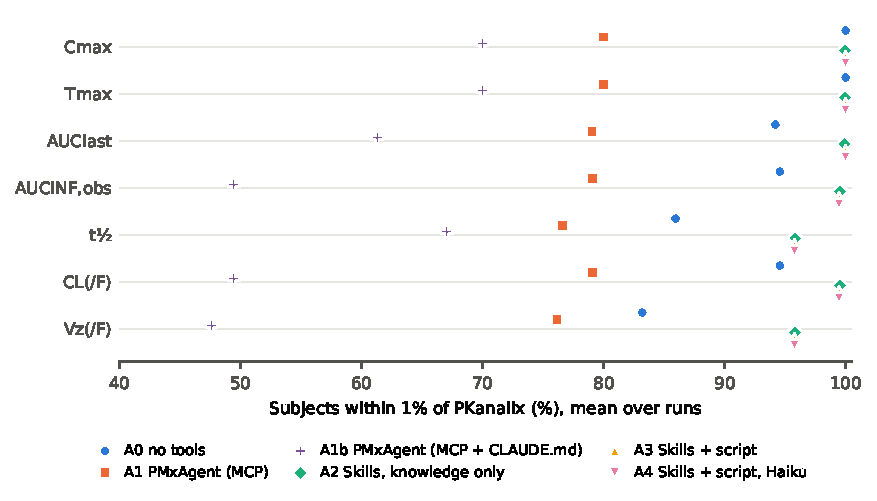
\includegraphics[width=\linewidth]{figures/fig_params_T1_nca.pdf}
\caption{T1 accuracy by parameter and arm (mean over runs). Each arm has its own marker shape.}
\label{fig:params}
\end{figure}

\subsection{T1: PMxAgent with its instruction file (A1b, post hoc)}
With PMxAgent's \texttt{CLAUDE.md} added (A1b), accuracy was \numToneAonebAcc\% (SD \numToneAonebAccSD,
$n=\numToneAonebN$; Table~\ref{tab:acc}). The agent called a PMxAgent tool in \numToneAonebPmxRuns\ of
\numToneAonebPmxKnown\ runs, against \numToneAonePmxRuns\ of \numToneAonePmxKnown\ for A1. In \numToneAonebUnscorable\
runs the results could not be matched to any subject and scored 0; without them A1b scored \numToneAonebAccPostHoc\%.
A1b$-$A1 was \numToneAonebVsAoneSecondaryDiff\ percentage points (95\% CI \numToneAonebVsAoneSecondaryCI;
Table~\ref{tab:secondary}): the mean was lower than A1's, and the interval is too wide to show a difference in either
direction. The Skills arms were more accurate than A1b (A2$-$A1b \numToneAtwoVsAonebSecondaryDiff,
\numToneAtwoVsAonebSecondaryCI; A3$-$A1b \numToneAthreeVsAonebSecondaryDiff, \numToneAthreeVsAonebSecondaryCI;
A4$-$A1b \numToneAfourVsAonebSecondaryDiff, \numToneAfourVsAonebSecondaryCI).

\begin{table}[t]
\centering\small
\caption{T1 secondary arm A1b (post hoc): comparisons of overall accuracy, as in Table~\ref{tab:stats}.}
\label{tab:secondary}
% generated by paper/tables.py - do not edit
\begin{tabular}{l c r c r c}
\toprule
Comparison & $n$ & Difference (pp) & 95\% CI & $p$ (perm.) & Within $\pm$1 pp \\
\midrule
A1b $-$ A1 & 10 vs 10 & $-$18.28 & $-$41.62 to $-$1.16 & 0.0681 & no \\
A2 $-$ A1b & 10 vs 10 & +18.70 & +1.55 to +42.06 & $<$0.0001 & no \\
A3 $-$ A1b & 10 vs 10 & +18.69 & +1.53 to +42.06 & $<$0.0001 & no \\
A4 $-$ A1b & 10 vs 10 & +18.69 & +1.53 to +41.28 & $<$0.0001 & no \\
\bottomrule
\end{tabular}

\end{table}

\subsection{T1: reproducibility}
A3 and A4 produced the same overall accuracy in every run (SD \numToneAthreeAccSD\ and \numToneAfourAccSD): across
\numToneAthreeN\ and \numToneAfourN\ runs there were \numToneAthreeDistinct\ and \numToneAfourDistinct\ distinct sets
of parameter values. Their output files formed \numToneAthreeDistinctFiles\ and \numToneAfourDistinctFiles\ distinct
sets, differing only in extra files such as plots and summaries. A0 varied from run to run (SD \numToneAzeroAccSD;
\numToneAzeroDistinct\ distinct value sets). A2 varied little in accuracy (SD \numToneAtwoAccSD) but gave
\numToneAtwoDistinct\ distinct value sets, because the agent wrote new code each time. A1, which also wrote its own
code, gave \numToneAoneDistinct\ distinct value sets. Value sets are counted over the runs that had a scorable file.

\subsection{T1: effort and cost}
The two PMxAgent arms (A1, A1b) needed the most turns and tool calls and the longest wall time (Table~\ref{tab:effort},
Figure~\ref{fig:cost}); part of the wall time reflects PMxAgent's amd64 containers running under emulation on the test
machine. A1b was the most expensive arm (\$\numToneAonebCost\ per run, against \$\numToneAoneCost\ for A1). A3 and A4
were the cheapest and fastest arms.

\begin{table}[t]
\centering\small
\caption{T1 effort per run (mean $\pm$ SD). Cost is Claude Code's list-price estimate; runs used a subscription.}
\label{tab:effort}
% generated by paper/tables.py - do not edit
\begin{tabular}{l r r r r r}
\toprule
Arm & Cost/run (USD) & Wall time (min) & Turns & Tool calls & Tool errors \\
\midrule
A0 & 0.381 $\pm$ 0.123 & 3.1 $\pm$ 1.8 & 11.8 $\pm$ 1.8 & 10.8 $\pm$ 1.8 & 0.9 $\pm$ 0.6 \\
A1 & 0.730 $\pm$ 0.138 & 5.2 $\pm$ 1.0 & 27.0 $\pm$ 6.9 & 26.0 $\pm$ 6.9 & 1.6 $\pm$ 1.8 \\
A1b & 1.012 $\pm$ 0.418 & 8.0 $\pm$ 4.2 & 28.2 $\pm$ 9.4 & 27.2 $\pm$ 9.4 & 1.8 $\pm$ 1.5 \\
A2 & 0.497 $\pm$ 0.087 & 3.8 $\pm$ 1.4 & 16.6 $\pm$ 2.9 & 14.6 $\pm$ 2.9 & 1.3 $\pm$ 0.7 \\
A3 & 0.198 $\pm$ 0.037 & 1.2 $\pm$ 0.3 & 12.5 $\pm$ 1.6 & 10.5 $\pm$ 1.6 & 0.1 $\pm$ 0.3 \\
A4 & 0.086 $\pm$ 0.018 & 1.1 $\pm$ 0.3 & 13.6 $\pm$ 3.9 & 11.6 $\pm$ 3.9 & 0.9 $\pm$ 0.7 \\
\bottomrule
\end{tabular}

\end{table}

\begin{figure}[t]
\centering
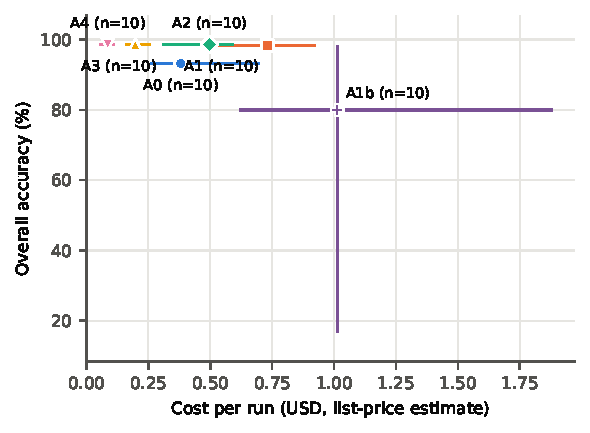
\includegraphics[width=0.62\linewidth]{figures/fig_cost_T1_nca.pdf}
\caption{T1 overall accuracy against cost per run. Markers are means across runs; bars span the minimum to maximum.}
\label{fig:cost}
\end{figure}

\subsection{T2: simulation case study}
Every run of every arm completed T2 and reported all three dose groups (Table~\ref{tab:t2}). On this workflow, the one
PMxAgent's tools were demonstrated on, A1 called a PMxAgent tool in \numTtwoAonePmxRuns\ of \numTtwoAonePmxKnown\
runs. Under the pre-specified check, the reported group means matched the run's own simulated data in
\numTtwoAthreeCons\% of comparisons for A3 and \numTtwoAtwoCons\% for A2, against \numTtwoAzeroCons\% for A0,
\numTtwoAoneCons\% for A1 and \numTtwoAfourCons\% for A4. Accepting either AUC rule (sensitivity analysis) raised A0 to
\numTtwoAzeroConsAny\% and A4 to \numTtwoAfourConsAny\%; A1 stayed at \numTtwoAoneConsAny\%, because in some of its
runs the reported mean AUC$_\mathrm{last}$ matched neither rule.

Because runs chose their own parameter values and units, Table~\ref{tab:t2} reports only whether EC$_{50}$ values
agreed. In \numTtwoAthreeEcModal\ of \numTtwoAthreeN\ A3 runs
the agent used the published monoclonal-antibody parameter set packaged in the Skills, the bundled simulation script and
the same seed, and these runs gave an identical EC$_{50}$. A2 had the same parameter set in its instructions but wrote
its own code (\numTtwoAtwoEcDistinct\ distinct values). Every A1 run used PMxAgent's default parameter set and the same
seed, yet A1 gave \numTtwoAoneEcDistinct\ distinct values, the largest group of identical values containing
\numTtwoAoneEcModal\ runs. The large differences came from the runs whose reported AUCs did not match their own
simulated data; the other runs differed only slightly, through the sampling times they chose. In A0 and A4 every run
gave a different value, and A4 reported EC$_{50}$ in different units from run to run.

PMxAgent's supplement reports an EC$_{50}$ of \numTtwoPmxEcClaude\ and \numTtwoPmxEcCursor\ h$\cdot\mu$g/mL from its
own two case-study runs, made with Claude and with Cursor \cite{bloomingdale2026pmxagent}. Converted to that unit, a
run's EC$_{50}$ was within 1\% of a published value in \numTtwoAthreeEcPmx\ of \numTtwoAthreeEcConv\ A3 runs,
\numTtwoAtwoEcPmx\ of \numTtwoAtwoEcConv\ A2 runs, \numTtwoAoneEcPmx\ of \numTtwoAoneEcConv\ A1 runs,
\numTtwoAzeroEcPmx\ of \numTtwoAzeroEcConv\ A0 runs and \numTtwoAfourEcPmx\ of \numTtwoAfourEcConv\ A4 runs
(Table~\ref{tab:t2}; descriptive, since the prompt fixes neither parameters nor sampling times).

\begin{table}[t]
\centering\small
\caption{T2 case study per arm. Completed: \texttt{results.json} with all three dose groups. Checked: runs whose
simulated data the scorer could read. Consistent: mean percentage of reported group means (AUC$_\mathrm{last}$,
$C_\mathrm{max}$) within 1\% of the means recomputed from the run's own simulated data (AUC$_\mathrm{last}$ by the
linear-up/log-down rule). $^\dagger$Either AUC rule accepted (sensitivity analysis). EC$_{50}$ values are compared at
three significant digits; the summary was chosen after the T2 data were seen. $^\S$Runs whose EC$_{50}$, converted to
h$\cdot\mu$g/mL, lies within 1\% of either value in PMxAgent's supplement, of the runs whose unit could be converted;
descriptive, chosen after the T2 data were seen.}
\label{tab:t2}
\resizebox{\linewidth}{!}{% generated by paper/tables.py - do not edit
\begin{tabular}{l r r r r r r r r}
\toprule
Arm & $n$ & Completed & Checked & Consistent (\%) & Either rule (\%)$^\dagger$ & Distinct EC$_{50}$ & Largest identical group & EC$_{50}$, h$\cdot\mu$g/mL$^\S$ \\
\midrule
A0 & 10 & 10 & 10 & 95.0 & 100.0 & 10 & 1 & 5.21--52.09 (10) \\
A1 & 10 & 10 & 10 & 80.0 & 80.0 & 5 & 3 & 86.69--1{,}843 (10) \\
A2 & 10 & 10 & 10 & 100.0 & 100.0 & 9 & 2 & 7.861--3{,}357 (10) \\
A3 & 10 & 10 & 10 & 100.0 & 100.0 & 2 & 9 & 9.361--2{,}127 (10) \\
A4 & 10 & 10 & 10 & 68.3 & 88.3 & 10 & 1 & 0.00011--49.81 (9) \\
\bottomrule
\end{tabular}
}
\end{table}

\subsection{T3: stress tasks}
A3 gave one set of parameter values in every run of each NCA stress task (Table~\ref{tab:t3acc}).
A2 was as accurate as A3 on T3a, T3b and T3e (A3$-$A2 within $\pm$1 point; Table~\ref{tab:t3stats}) but gave several
value sets per task. Without tools, accuracy was lower than A3's on every NCA stress task (A0$-$A3 from
\numTthreebAzeroVsAthreeDiff\ on T3b to \numTthreeaAzeroVsAthreeDiff\ on T3a). A3 was equivalent to A1 on T3a, T3c
and T3e and more accurate on T3b (A3$-$A1 \numTthreebAthreeVsAoneDiff, \numTthreebAthreeVsAoneCI). A1 called a PMxAgent
tool only on T3a (\numTthreeaAonePmxRuns\ of \numTthreeaAonePmxKnown\ runs).

The smaller model with the script (A4) matched A3 on T3b and T3e, again with one value set per task, but not on T3a
(A4$-$A3 \numTthreeaAfourVsAthreeDiff, \numTthreeaAfourVsAthreeCI), where its results varied between runs, or on T3c
(\numTthreecAfourVsAthreeDiff), where the same subset of results was wrong in every run. Unlike on T1, many of A4's
$\lambda_z$-dependent errors on these two tasks were in subjects whose points matched PKanalix
(\numTthreecAfourLzErrMatch\ of \numTthreecAfourLzErr\ on T3c, \numTthreeaAfourLzErrMatch\ of \numTthreeaAfourLzErr\ on
T3a).

On T3d (exploratory comparisons), A0, A2 and A3 reported all three typical values within 1\% of the analytical solution
in every run. A1 scored \numTthreedAoneAcc\% and A4 \numTthreedAfourAcc\%; in each run that lost points,
$t_\mathrm{max}$ differed from the analytical value by more than 1\%. A1 called a PMxAgent tool in
\numTthreedAonePmxRuns\ of \numTthreedAonePmxKnown\ T3d runs: the agent wrote its own simulation code.

\begin{table}[t]
\centering\small
\caption{T3 accuracy per arm (mean over 5 runs). NCA tasks (T3a, T3b, T3c, T3e): the T1 metric. T3d: percentage of
the three typical values within 1\% of the analytical solution. Sets: distinct sets of parameter values across runs.}
\label{tab:t3acc}
\resizebox{\linewidth}{!}{% generated by paper/tables.py - do not edit
\begin{tabular}{l r r r r r r r r r r }
\toprule
 & \multicolumn{2}{c}{T3a} & \multicolumn{2}{c}{T3b} & \multicolumn{2}{c}{T3c} & \multicolumn{2}{c}{T3d} & \multicolumn{2}{c}{T3e} \\
\cmidrule(lr){2-3} \cmidrule(lr){4-5} \cmidrule(lr){6-7} \cmidrule(lr){8-9} \cmidrule(lr){10-11}
Arm & Acc. & Sets & Acc. & Sets & Acc. & Sets & Acc. & Sets & Acc. & Sets \\
\midrule
A0 & 92.93 & 4 & 95.53 & 4 & 93.63 & 3 & 100.00 & -- & 93.21 & 4 \\
A1 & 98.68 & 4 & 92.88 & 5 & 98.68 & 3 & 93.33 & -- & 98.24 & 3 \\
A2 & 98.68 & 4 & 97.32 & 5 & 98.21 & 5 & 100.00 & -- & 98.68 & 4 \\
A3 & 98.68 & 1 & 97.43 & 1 & 98.68 & 1 & 100.00 & -- & 98.64 & 1 \\
A4 & 92.46 & 4 & 97.43 & 1 & 85.51 & 1 & 73.34 & -- & 98.64 & 1 \\
\bottomrule
\end{tabular}
}
\end{table}

\begin{table}[t]
\centering\small
\caption{T3 comparisons of mean accuracy (percentage points; 5 vs 5 runs; 95\% percentile bootstrap CI).
$^\ddagger$Exploratory (T3d is not an NCA task); the NCA-task comparisons were pre-specified.}
\label{tab:t3stats}
% generated by paper/tables.py - do not edit
\begin{tabular}{l l r c c}
\toprule
Task & Comparison & Difference (pp) & 95\% CI & Within $\pm$1 pp \\
\midrule
T3a & A2 $-$ A1 & +0.00 & +0.00 to +0.00 & yes \\
T3a & A3 $-$ A1 & +0.00 & +0.00 to +0.00 & yes \\
T3a & A3 $-$ A2 & +0.00 & +0.00 to +0.00 & yes \\
T3a & A4 $-$ A3 & $-$6.22 & $-$12.50 to +0.00 & no \\
T3a & A0 $-$ A3 & $-$5.75 & $-$7.02 to $-$4.48 & no \\
\addlinespace
T3b & A2 $-$ A1 & +1.24 & +0.94 to +1.55 & no \\
T3b & A3 $-$ A1 & +1.35 & +1.09 to +1.63 & no \\
T3b & A3 $-$ A2 & +0.11 & +0.00 to +0.22 & yes \\
T3b & A4 $-$ A3 & +0.00 & +0.00 to +0.00 & yes \\
T3b & A0 $-$ A3 & $-$1.90 & $-$2.36 to $-$1.67 & no \\
\addlinespace
T3c & A2 $-$ A1 & $-$0.47 & $-$1.30 to +0.00 & no \\
T3c & A3 $-$ A1 & +0.00 & +0.00 to +0.00 & yes \\
T3c & A3 $-$ A2 & +0.47 & +0.00 to +1.30 & no \\
T3c & A4 $-$ A3 & $-$13.17 & $-$13.17 to $-$13.17 & no \\
T3c & A0 $-$ A3 & $-$5.05 & $-$6.72 to $-$2.61 & no \\
\addlinespace
T3d$^\ddagger$ & A2 $-$ A1 & +6.67 & +0.00 to +20.00 & no \\
T3d$^\ddagger$ & A3 $-$ A1 & +6.67 & +0.00 to +20.00 & no \\
T3d$^\ddagger$ & A3 $-$ A2 & +0.00 & +0.00 to +0.00 & yes \\
T3d$^\ddagger$ & A4 $-$ A3 & $-$26.67 & $-$33.33 to $-$13.33 & no \\
T3d$^\ddagger$ & A0 $-$ A3 & +0.00 & +0.00 to +0.00 & yes \\
\addlinespace
T3e & A2 $-$ A1 & +0.44 & +0.38 to +0.53 & yes \\
T3e & A3 $-$ A1 & +0.40 & +0.35 to +0.49 & yes \\
T3e & A3 $-$ A2 & $-$0.04 & $-$0.06 to $-$0.01 & yes \\
T3e & A4 $-$ A3 & +0.00 & +0.00 to +0.00 & yes \\
T3e & A0 $-$ A3 & $-$5.43 & $-$5.90 to $-$4.49 & no \\
\bottomrule
\end{tabular}

\end{table}

\subsection{T2 and T3: cost}
A3 cost less per run than A1 on T2 and on every T3 task, and A4 was the cheapest arm on T3a, T3b, T3c and T3e
(Table~\ref{tab:cost23}).

\begin{table}[t]
\centering\small
\caption{T2 and T3 mean list-price cost per run (USD).}
\label{tab:cost23}
% generated by paper/tables.py - do not edit
\begin{tabular}{l r r r r r r }
\toprule
Arm & T2 & T3a & T3b & T3c & T3d & T3e \\
\midrule
A0 & 0.23 & 0.58 & 0.46 & 0.63 & 0.12 & 0.56 \\
A1 & 0.66 & 1.12 & 0.79 & 0.82 & 0.18 & 0.86 \\
A2 & 0.54 & 0.62 & 0.51 & 0.43 & 0.21 & 0.44 \\
A3 & 0.24 & 0.54 & 0.18 & 0.37 & 0.16 & 0.23 \\
A4 & 0.30 & 0.20 & 0.09 & 0.19 & 0.12 & 0.07 \\
\bottomrule
\end{tabular}

\end{table}

\subsection{Infrastructure}
PMxAgent needs \numInfraPmxagentService\ services running before the agent starts (a container engine and
\numInfraPmxagentContainer\ containers) and opens \numInfraPmxagentPort\ host ports; the Skills need
\numInfraSkillsService\ services and \numInfraSkillsPort\ ports (Table~\ref{tab:infra}). Setting up needs
\numInfraPmxagentSetup\ steps for PMxAgent and \numInfraSkillsSetup\ for the Skills. PMxAgent's repository holds
\numInfraPmxagentLines\ maintained lines (\numInfraPmxagentTool\ of tool code and \numInfraPmxagentServing\ of serving
and infrastructure code), the Skills \numInfraSkillsLines\ (\numInfraSkillsTool\ in the bundled scripts). PMxAgent's
extra code also provides OAuth authorisation, typed input validation, a server any MCP client can use, a containerised R
environment on a digest-pinned base, and tests and release pipelines for these; the Skills rely on the user's own R
installation, counted as one setup step however long it takes.

\begin{table}[t]
\centering\small
\caption{Infrastructure footprint per stack. Lines are non-blank, non-comment lines in the repository (Python
docstrings count as lines, PMxAgent's Plumber route annotations as comments); documentation and licence files are not
counted. PMxAgent's \texttt{CLAUDE.md} is loaded only in arm A1b. PMxAgent's larger code base also provides OAuth,
typed input validation, support for any MCP client and a container environment, which the Skills do not.
$^a$From a machine with Claude Code installed; each step is listed in \texttt{results/infra.csv}.
$^b$API router, MCP server, container and compose files, dependency lists and CI workflows.}
\label{tab:infra}
% generated by paper/tables.py - do not edit
\begin{tabular}{l r r}
\toprule
 & PMxAgent 1.0.0 & Agent Skills \\
\midrule
Services running before the agent starts & 3 & 0 \\
Containers & 2 & 0 \\
Host network ports & 2 & 0 \\
Setup steps$^a$ & 5 & 3 \\
\addlinespace
Maintained lines of code \\
\quad Tool code (Skills: bundled scripts) & 3{,}920 & 634 \\
\quad Serving and infrastructure code$^b$ & 1{,}000 & 0 \\
\quad Tests & 1{,}706 & 308 \\
\quad Agent instructions (\texttt{CLAUDE.md}; \texttt{SKILL.md}) & 663 & 214 \\
\quad Total & 7{,}289 & 1{,}156 \\
\bottomrule
\end{tabular}

\end{table}

% ---------------------------------------------------------------------------------------------------------------
\section{Discussion}
On PMxAgent's own NCA benchmark, the two properties that motivate its architecture separated cleanly. Instructions on
choosing the terminal phase and deriving parameters raised accuracy from \numToneAzeroAcc\% to \numToneAtwoAcc\%
while the agent still wrote its own code; only the arms that called a tested script returned identical values in every
run. Neither property needed a container, an API server or MCP.

Our results agree with the published ones where the two studies overlap. Without tools, the same model scored 94.5\%
in PMxAgent's evaluation \cite{bloomingdale2026pmxagent} and \numToneAzeroAcc\% here, and in both the losses fell on the
$\lambda_z$-dependent parameters. With Skills the agent reached \numToneAtwoAcc\% (instructions only) and
\numToneAthreeAcc\% (with the script), level with the 98.3\% published for PMxAgent, without its server. What remained
with the script was the choice of terminal phase: none of A3's $\lambda_z$-dependent errors on T1 occurred in a subject
whose terminal phase used the same number of points as PKanalix. Closing the last gap to PKanalix is therefore a
question of the point-selection rule, not of the infrastructure around the calculation.

Earlier studies found that LLM output, including generated code, varied between repeats of the same prompt
\cite{shin2023chatgptpk,shin2024nonmem}, and PMxAgent's authors found the same for agents that wrote new NCA code in
each run \cite{bloomingdale2026pmxagent}. Here too the values varied whenever the agent wrote its own code. A0 gave \numToneAzeroDistinct\ and
A2 \numToneAtwoDistinct\ distinct sets of values in 10 runs. A2 shows that good instructions narrow the spread of
accuracy (SD \numToneAtwoAccSD) without removing the variation in the values themselves. Fixed code removed it, as
PMxAgent's design intends, but it did not have to sit behind a server: a local script was enough.

Offered PMxAgent's tools, the agent called them in \numToneAonePmxRuns\ of \numToneAonePmxKnown\ T1 runs, and in
\numNcaAonePmxRuns\ of \numNcaAonePmxKnown\ runs over the five NCA tasks; it preferred to write its own PKNCA code. A
tool stack only helps if the agent calls it. Our A1 results therefore test neither PMxAgent's NCA endpoint nor the
run-to-run identity reported for it \cite{bloomingdale2026pmxagent}. The \numToneAoneUnscorable\ A1 runs that scored 0 show a
second cost of agent-written code: an output that omits the subject identifier is unusable however accurate the
calculations. The agent may have bypassed the tools because the NCA tool's API description omits the multi-drug input
this benchmark needs. Adding PMxAgent's instruction file, which documents that input (A1b, post hoc), raised tool use to
\numToneAonebPmxRuns\ of \numToneAonebPmxKnown\ runs, but not mean accuracy, and \numToneAonebUnscorable\ runs again
gave results that could not be matched to subjects.

The stress tasks gave the same picture under harder conditions: with the script, the larger model returned one set of
values in every run of each NCA stress task, whether the input was a messy workbook, carried a below-quantification
rule, mixed units or was five times larger, and without tools the agent was less accurate on each. T2 sets a limit on
the reproducibility claim: fixed code gives identical values only when the steps around it are fixed too. A1 called
PMxAgent's tools in every T2 run with the same default parameters and seed, yet its EC$_{50}$ varied, because some runs
reported AUCs that did not match their own simulated data and the others chose different sampling times. A3 runs that
used the packaged parameter set and script, which fix those steps, gave identical values. In T3d, outside PMxAgent's
simulation tool, A0 and A2 solved the oral model in every run with their own code, so T3d tested the agent rather than
any tool: the Skills reached a step outside PMxAgent's tool set, but so did the agent without them.

The smaller model matched the larger one with the script on T1, T3b and T3e, but not on T3a, T3c or T3d. On T3c it made
the same error in every run, mostly in subjects whose terminal points matched PKanalix: the script made its results
reproducible, not correct. The work around the script, such as preparing its input from a messy workbook or from
mixed units, still depended on the model.

This does not make MCP redundant. An MCP server works with any compatible client, validates typed inputs at the tool
boundary, and can be deployed once for many users in a controlled environment; Skills as used here run on the user's
own machine with the user's own R installation. Much of PMxAgent's larger code base (Table~\ref{tab:infra}) pays for
these properties, which can matter more than setup cost in a regulated, multi-user deployment.

The next study should measure the server's own contribution, which ours could not. It would run the same arms with a
prompt that names PMxAgent's tools, so that A1 measures the endpoint rather than the agent's choice to bypass it, and
repeat them on a second MCP-capable client and a second model family. A benchmark with analytical $\lambda_z$ truth
would also separate a wrong point-selection rule from a disagreement with PKanalix.

\subsection{Limitations}
\emph{Benchmark and models.} One benchmark source was used, with PKanalix as the reference rather than an analytical
truth, and accuracy with the Skills was near a ceiling (\numToneAthreeAcc\% on T1), where small real differences could
not be detected. Only Claude models in one client were tested, so the finding that a small model suffices with a script
may not transfer. Cost is a list-price estimate, and PMxAgent's containers ran under emulation, which lengthened A1's
wall time but not its turns or tool calls.

\emph{Arms.} We wrote the Skills, with an AI coding assistant, from package documentation, and froze them before any
run without comparing their output with PKanalix; they are still not independent of the study. If our NCA conventions
match PKanalix's more closely than an independent author's would, A2--A4 are favoured on the NCA tasks, though not on
T3d, whose reference is analytical. A1 reflects PMxAgent as offered to this client and model and probably understates
its NCA endpoint, whose published output scored 98.3\% with our scorer. That the omitted multi-drug input explains the
bypass is a hypothesis; A1b, which tests it, was specified after the A0--A4 T1 results were known, and its instruction
file was written by PMxAgent's authors for this benchmark's workflow.

\emph{T1 protocol.} The T1 statistical comparisons were specified after the first T1 runs, the analysis without
unscorable runs after seeing the scores, and the split of $\lambda_z$ errors by terminal-point match after all results
were seen. The user-global instruction file was loaded in every T1 arm except A1 runs 4--10 and all A1b runs. A1 runs
4--10 and the A1b runs were made about eight weeks after the other T1 runs, with the same Claude Code version, model
and container images; the pre-specified split by isolation regime shows how much A1's result depends on this.

\emph{T2 and T3.} T2 has no reference answer: it shows completion, internal consistency and agreement between runs, not
correctness. Its EC$_{50}$ summaries were defined after the data were seen, and the scorer's reading of the agents'
files was hand-checked on \numTtwoParserN\ of the \numTtwoRuns\ runs. Within A0 on T2, the first runs used a less
restrictive permission mode without the environment scrub of the later ones; no tool call was denied in either. T3 had
5 runs per arm, so its intervals are wide, and its T3d comparisons are exploratory. The T3 prompts, unlike T1's, stated
how to identify subjects, so the failure that cost A1 \numToneAoneUnscorable\ T1 runs could not recur there. A1 runs
of T2 and T3 made before PMxAgent's shared folders were emptied were excluded and repeated. T2 and T3 ran on a later
Claude Code version than T1 and over two subscription accounts, with the same model and version within a task, so
comparisons within a task are not affected.

\section{Conclusions}
On PMxAgent's NCA benchmark and four harder NCA inputs, Agent Skills with a bundled, tested script were at least as
accurate as the same agent offered an MCP platform, gave identical parameter values in every run with the larger model,
and cost less without server infrastructure; offered only the platform's tools, the agent rarely used them. In
simulation, identical values needed the whole workflow fixed, not only the calculation. Pharmacometric agent designs
should test instructions, fixed code and serving infrastructure separately before adopting the heavier stack.

% ---------------------------------------------------------------------------------------------------------------
\section*{Data and code availability}
Code, frozen Skills, scorer and per-run results:
\url{https://github.com/heyiamnotacoder/pmxagent-skills-benchmark}, release \texttt{v1.0-preprint}. Raw transcripts, outputs and logs
for every run, including failed runs: Zenodo, version 2, \href{https://doi.org/10.5281/zenodo.24478971}{doi:10.5281/zenodo.24478971}
\cite{zenodo_evidence}; all versions: \href{https://doi.org/10.5281/zenodo.23019417}{doi:10.5281/zenodo.23019417}. Benchmark data are from the supporting information of \cite{bloomingdale2026pmxagent}
(CC BY-NC); PKanalix reference values are not redistributed.

\section*{Use of AI tools}
Apart from the agents under test, Claude Code (Anthropic), running Claude models, was used to write the benchmark
harness, scorer, Skills and analysis scripts, to draft this manuscript, and to revise its text for length and clarity.
The author checked all code, results and text, and takes full responsibility for their accuracy, integrity and
originality. No AI tool is listed as an author.

\section*{Author contributions}
D.P. (sole author): conceptualization, methodology, software, investigation, formal analysis, data curation,
visualization, writing (original draft), writing (review and editing).

\section*{Competing interests}
The author declares no competing interests.

\section*{Funding}
This research received no specific grant from any funding agency in the public, commercial or not-for-profit sectors.

\bibliographystyle{unsrtnat}
\bibliography{references}
\end{document}
